\documentclass[10pt,english]{article}
\usepackage{babel,amsmath,amsfonts,amssymb,color,fancybox}
\usepackage[latin1]{inputenc}
\usepackage[a4paper, inner=2.5cm, outer=2.5cm, top=2.0cm, bottom=2cm, bindingoffset=0cm]{geometry}
\usepackage{graphicx}

%\usepackage{times}                  % stile delle sections

\newcommand{\reals}{\mathbf{R}}
\parindent=0pt \parskip=3pt
%
\title{Review of ``Decentralized Proximal Gradient Algorithms With Linear Convergence Rates''}
\date{version: \today}%Meeting held on: April the 2nd}
\author{P. Gatt}
\begin{document}

\maketitle
%\small

\section{Introduction}

\subsection{Summary of the paper}

The paper studies decentralized composite optimization over a static undirected network.
Each agent has a local smooth strongly convex function, and all agents share one common nonsmooth regularizer.
The key contribution is a primal-dual unified decentralized algorithm (UDA), then its proximal extension (PUDA).
This framework recovers several known methods by choosing specific consensus matrices: exact diffusion, NIDS, ATC tracking, Aug-DGM, and also non-ATC variants such as EXTRA/DLM.
The main theoretical result is global linear convergence of PUDA to the exact minimizer under strong convexity, smoothness, and matrix conditions.
An important practical insight is that for the class with $C=0$ (including exact diffusion), the step-size bound is as large as centralized proximal gradient descent: $\mu < 2/\delta$.
The paper also gives a lower-bound result for the harder case where each agent has a different nonsmooth term $R_k$: in that regime, one cannot guarantee global linear convergence in the worst case for proximal-gradient-based decentralized updates.
Therefore, the paper clarifies both what is achievable (common nonsmooth term) and what is fundamentally limited (agent-specific nonsmooth terms).
Compared with course baselines, this work extends gradient-tracking/exact-diffusion ideas to composite objectives with linear rates.

\subsection{Problem formulation}

Using course notation, the target problem is
\[
\min_{w\in\reals^m} F(w)
= \frac{1}{K}\sum_{k=1}^K f_k(w) + r(w),
\]
where $f_k$ is smooth strongly convex and $r$ is convex, possibly nonsmooth.

To decentralize, each agent keeps a local copy $w_k$ and we stack
\[
W=\mathrm{col}\{w_1,\dots,w_K\}\in\reals^{Km}.
\]
Define
\[
J(W)=\frac{1}{K}\sum_{k=1}^K f_k(w_k),\qquad
R(W)=\frac{1}{K}\sum_{k=1}^K r(w_k).
\]
Consensus is encoded by a matrix $B$ such that
\[
BW=0 \iff w_1=\cdots=w_K.
\]
Then the constrained decentralized form is
\[
\min_{W\in\reals^{Km}} J(W)+R(W)\quad \text{s.t.}\quad BW=0.
\]

For the smooth case ($R=0$), the paper writes a saddle-point problem and proposes a primal-dual recursion in variables $(W_i,Y_i,Z_i)$.
For the composite case, PUDA updates are
\begin{align*}
Z_i &= (I-C)W_{i-1} - \mu \nabla J(W_{i-1}) - B Y_{i-1},\\
Y_i &= Y_{i-1} + B Z_i,\\
W_i &= \mathrm{prox}_{\mu R}(\bar A Z_i).
\end{align*}
Choosing $(\bar A,B,C)$ gives specific algorithms (Prox-ED, Prox-ATC I, Prox-ATC II, etc.).

In my kernel experiment, $w=\alpha\in\reals^m$ is the Nystr\"om coefficient vector and each local $f_k$ is quadratic:
\[
f_k(\alpha)=\frac12\|M_k\alpha-y_k\|^2+\frac{\sigma^2}{2K}\alpha^\top K_{mm}\alpha+\frac{\nu}{2K}\|\alpha\|^2,
\]
with common nonsmooth term $r(\alpha)=\lambda\|\alpha\|_1$ for the PUDA test.

\subsection{Assumptions}

Main assumptions used for linear convergence are:
\begin{itemize}
\item \textbf{Cost regularity:} each $f_k$ is differentiable, $\nu$-strongly convex, and has $\delta$-Lipschitz gradient:
\[
\langle \nabla f_k(u)-\nabla f_k(v),u-v\rangle\ge \nu\|u-v\|^2,\quad
\|\nabla f_k(u)-\nabla f_k(v)\|\le \delta\|u-v\|.
\]
\item \textbf{Common nonsmooth term:} $r$ is proper, lower-semicontinuous, convex.
\item \textbf{Consensus matrices:} $B$ and $C$ satisfy
\[
BW=0 \iff \text{consensus},\qquad C=0\ \text{or}\ CW=0 \iff BW=0.
\]
\item \textbf{Technical matrix condition (ATC analysis):}
\[
\bar A^2 \preceq I-B^2,\qquad 0\preceq C\prec 2I.
\]
\end{itemize}

For ATC forms, this condition is met when the graph mixing matrix has eigenvalues in $[0,1]$ (or after the usual shift $A\leftarrow (I+A)/2$).
These assumptions are stronger than some alternatives in the literature, but they lead to simple, network-friendly step-size bounds of order $O(1/\delta)$.

\section{Result: theory and practice}

\subsection{Theory}

The key result is linear convergence of the PUDA error dynamics.
Let $(W^\star,Y^\star,Z^\star)$ be the fixed point (with $W^\star=1_K\otimes w^\star$) and define errors
\[
\widetilde W_i=W_i-W^\star,\quad
\widetilde Y_i=Y_i-Y^\star,\quad
\widetilde Z_i=Z_i-Z^\star.
\]
Under the assumptions above, if
\[
\mu < \frac{2-\sigma_{\max}(C)}{\delta},
\]
then
\[
\|\widetilde W_i\|_Q^2+\|\widetilde Y_i\|^2
\le
\gamma\left(\|\widetilde W_{i-1}\|_Q^2+\|\widetilde Y_{i-1}\|^2\right),
\]
with
\[
\gamma=\max\left\{1-\mu\nu\left(2-\sigma_{\max}(C)-\mu\delta\right),\;1-\sigma_{\min}(B^2)\right\}<1.
\]
Hence the method converges geometrically to the exact solution.

Interpretation:
\begin{itemize}
\item The first term in $\gamma$ is an optimization term (condition number/step size).
\item The second term is a network term (spectral gap of $B^2$).
\end{itemize}
For $C=0$ (exact diffusion / Prox-ED class), the bound becomes $\mu<2/\delta$, independent of the network, matching centralized proximal gradient admissible steps.

The second theoretical message is a lower bound for the case $\frac1K\sum_k (f_k(w)+r_k(w))$ with different nonsmooth $r_k$.
In worst case, for decentralized methods using one gradient and one proximal call per iteration, global linear convergence cannot be guaranteed dimension-independently.
This explains why the common-regularizer structure is central to the linear-rate claim.

\subsection{Practice}

The experimental comparison includes DGD, Gradient Tracking, and three PUDA instances from Appendix A (Prox-ED, Prox-ATC I, Prox-ATC II).
The study is reported in two regimes:
\begin{itemize}
\item smooth setting ($\lambda=0$), with centralized smooth reference;
\item composite nonsmooth setting ($\lambda>0$), with centralized $\ell_1$-regularized reference.
\end{itemize}

Experimental setup: Nystr\"om kernel regression ($n=100$, $m=20$, $K=5$ agents, cycle graph, $\sigma=0.5$, $\nu=1$).
From data, $\delta=232.333$ and for ATC-II the theorem bound is $\mu<(2-\sigma_{\max}(I-A))/\delta=0.004715$.
The value $\mu=0.004$ is used for PUDA variants (inside the bound).

\textbf{Smooth case ($\lambda=0$), final error $\|\bar\alpha_t-\alpha^\star\|_2$:}
\begin{center}
\begin{tabular}{lc}
\hline
Algorithm & Final error \\
\hline
DGD & $1.101\times 10^{-1}$ \\
Gradient Tracking & $1.801\times 10^{-2}$ \\
Prox-ED (PUDA) & $5.787\times 10^{-3}$ \\
Prox-ATC I (PUDA) & $5.795\times 10^{-3}$ \\
Prox-ATC II (PUDA) & $5.795\times 10^{-3}$ \\
\hline
\end{tabular}
\end{center}

\textbf{Nonsmooth case ($\lambda=10^{-3}$), final error $\|\bar\alpha_t-\alpha^\star_{\ell_1}\|_2$:}
\begin{center}
\begin{tabular}{lc}
\hline
Algorithm & Final error \\
\hline
Prox-ED & $9.122\times 10^{-3}$ \\
Prox-ATC I & $9.130\times 10^{-3}$ \\
Prox-ATC II & $9.129\times 10^{-3}$ \\
\hline
\end{tabular}
\end{center}

These results are consistent with the paper: PUDA variants converge quickly with near-identical rates in this setup; they significantly outperform DGD, and improve over GT in smooth mode.

\begin{figure}[h]
\centering
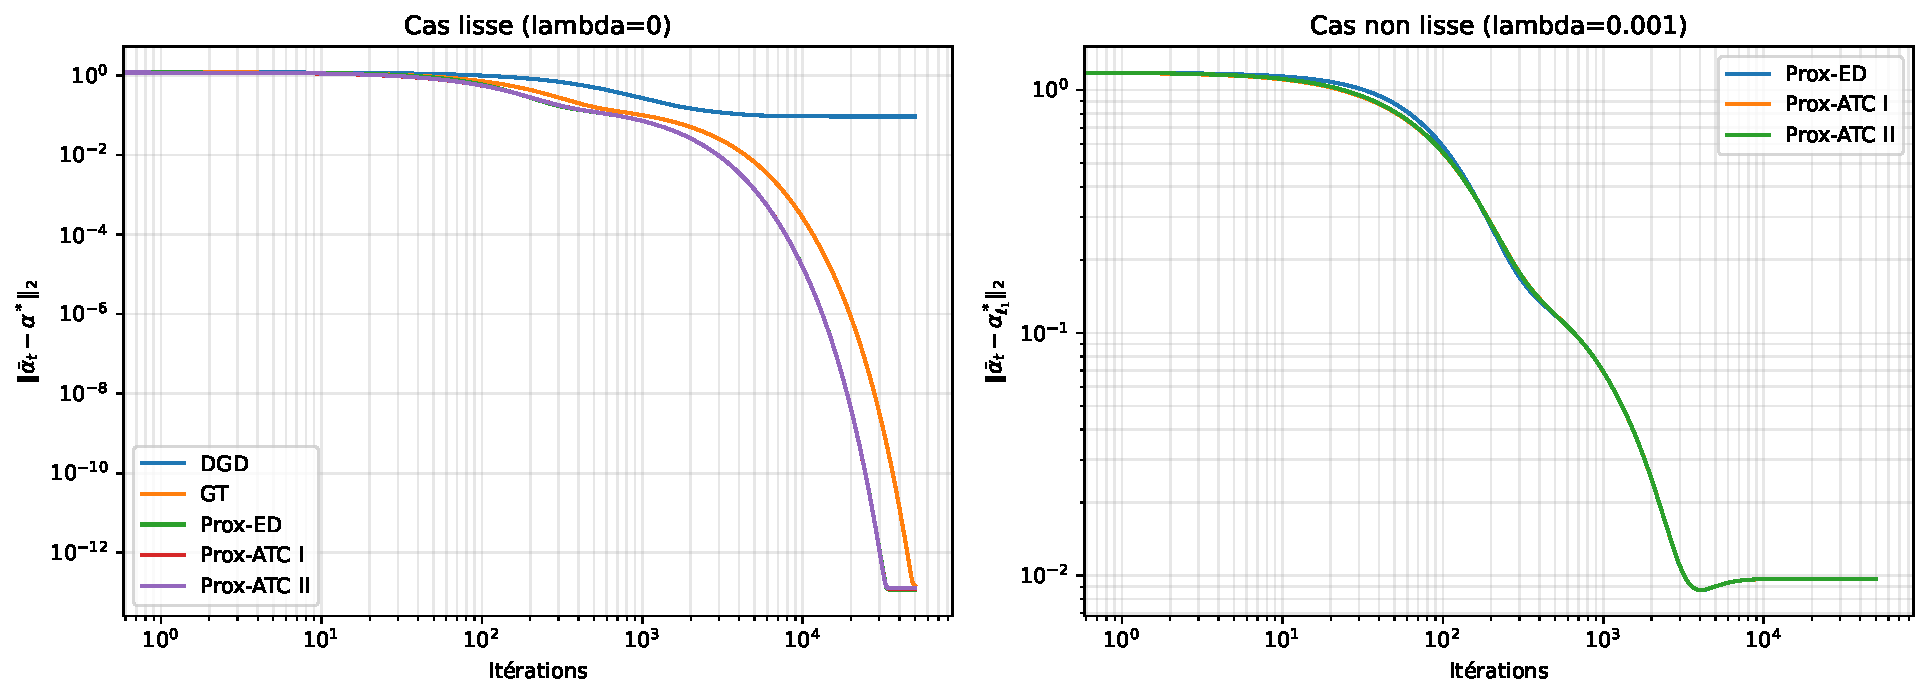
\includegraphics[width=\linewidth]{puda_comparison.pdf}
\caption{Convergence curves of the reported experiment (left: smooth, right: nonsmooth).}
\end{figure}

\section{Conclusion}

This paper is a useful bridge between course algorithms and current decentralized composite optimization theory.
It gives one primal-dual template that explains many existing recursions by matrix choices, instead of treating each algorithm separately.
For practice, the main value is the linear-rate guarantee with proximal terms when the nonsmooth regularizer is common across agents.
The step-size condition is also practically appealing, especially the $C=0$ case where $\mu<2/\delta$ matches centralized scaling.
The lower-bound section is equally important: if regularizers are agent-specific, linear convergence cannot be expected in worst case for this algorithmic class.
So the paper not only proposes a stronger method, it also clarifies the structural limits of the problem class.
In the kernel project experiment, PUDA-family methods are robust and faster than DGD, and competitive/superior to GT, while preserving exactness for composite objectives.

\end{document}
